\documentclass[conference]{IEEEtran}
\usepackage{amsmath,amssymb}
\usepackage{graphicx}
\usepackage{booktabs}
\usepackage{array}
\usepackage{url}
\usepackage{xurl}
\usepackage[colorlinks=true,linkcolor=black,citecolor=black,urlcolor=blue]{hyperref}
\usepackage{tikz}
\usetikzlibrary{arrows.meta,positioning}
\usepackage{balance}

\graphicspath{{figures/}}

\begin{document}

\title{AIRE: AI Reliability \& Evaluation Engine\\
\large Replayable Trace-Based Evaluation and Regression Testing for LLM and RAG Systems}

\author{\IEEEauthorblockN{Vaibhav Mahore}
\IEEEauthorblockA{\textit{Department of Mathematics and Computing}\\
\textit{Indian Institute of Science, Bangalore, India}\\
mvaibhav@iisc.ac.in}}

\maketitle

\begin{abstract}
Evaluating large language model (LLM) applications differs fundamentally from
testing conventional software: outputs are nondeterministic, no single
correct answer exists for most prompts, every evaluation may incur API cost,
and model behavior drifts under the provider's control. This paper presents
AIRE (AI Reliability \& Evaluation Engine), a system that separates system
execution from system evaluation. A system under test (SUT) is invoked once
per case; each invocation is recorded as a validated, schema-constrained
trace (answer, retrieved documents, timed spans, token usage with explicit
source labeling, errors). All downstream analysis (13 deterministic
metrics, a first-match failure taxonomy, and a direction-aware regression
engine with relative thresholds and per-case attribution) operates on the
stored traces and never re-runs the system. We demonstrate the engine on a
26-case retrieval-augmented-generation (RAG) suite over a 12-document
corpus with three deterministic SUT versions, in which the engine catches an
intentional ``fluent but uncited'' regression (lexical groundedness
0.57 to 0.00, ungrounded failure count +22) while confirming retrieval
improvements (recall 0.73 to 0.91), and on a live Gemini 2.5 Flash run of
the same suite, which improves abstention (0.0 to 1.0) and groundedness (0.57
to 1.0) at 15.3\,s per case and roughly 605 tokens per case. The live run
also illustrates the engine's operational value: six provider rate-limit
failures are recorded and classified rather than silently absorbed. AIRE's
groundedness metric is a lexical citation-overlap proxy, not semantic
entailment, and its deterministic responder is a reproducible harness rather
than a language model; both distinctions are stated and their consequences
analyzed.
\end{abstract}

\begin{IEEEkeywords}
LLM evaluation, RAG, observability, tracing, regression testing, groundedness, reliability engineering
\end{IEEEkeywords}

\section{Introduction}
Testing an LLM application with conventional assertions fails for five
reasons. (1) \emph{Nondeterminism}: identical prompts can yield different,
equally acceptable answers. (2) \emph{Absence of an oracle}: most prompts
have no single correct output, so equality assertions are inapplicable.
(3) \emph{Cost and latency}: every evaluation step may be a billable API
call taking seconds. (4) \emph{Drift}: providers may change model behavior
behind a stable model name. (5) \emph{Hidden failure modes}: a system can be
confidently wrong (hallucination) or right for unsupported reasons
(ungrounded), neither of which an \texttt{assert} detects.

The practical consequence is that teams change a prompt, a retriever, or a
model and cannot say systematically what improved or regressed. AIRE
addresses this with one design decision: \emph{run the system once, store
validated traces, and perform all evaluation and comparison on the stored
records}. Evaluation thereby becomes replayable (new metrics run at zero
API cost), fair (both versions are scored on identical stored outputs),
auditable (every score is traceable to a recorded answer and its evidence),
and safe from silent re-execution, which would inject nondeterminism into
the comparison itself.

This paper's contributions are: (1) a trace schema and storage format with
write-time validation (Section~III); (2) a metric suite of 13 deterministic
measures spanning answer quality, citation behavior, retrieval, tool use,
and operational cost (Section~IV); (3) a first-match failure taxonomy and a
direction-aware regression engine with scale-free relative thresholds and
per-case attribution (Section~V); (4) a controlled three-version RAG
demonstration including an intentional quality regression that the engine
detects, and a live evaluation of the same suite with a frontier LLM
(Section~VI); and (5) an explicit account of the evaluator's own limits and
of two reliability bugs the harness surfaced during development
(Section~VII).

\section{System Overview}
AIRE's pipeline separates execution from evaluation (Fig.~\ref{fig:pipe}).
The upper path runs once: an evaluation dataset (JSONL, one case per line)
drives a SUT; each invocation is wrapped into a \emph{Trace} by the runner,
which adds timeout enforcement and bounded retries. The lower path is pure
computation over stored records: the evaluation engine computes per-case
metrics and aggregate statistics, the failure classifier assigns each case
at most one category, and the regression engine compares two evaluated runs.
Reports are static, self-contained HTML files.

\begin{figure}[t]
\centering
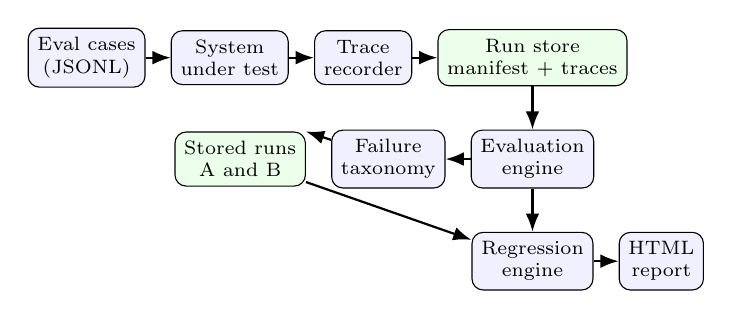
\begin{tikzpicture}[node distance=3.2mm, every node/.style={font=\scriptsize},
  box/.style={draw, rounded corners, fill=blue!6, minimum height=6.5mm, align=center},
  data/.style={box, fill=green!8},
  arr/.style={-{Latex}, thick}]
\node[box] (cases) {Eval cases\\(JSONL)};
\node[box, right=of cases] (sut) {System\\under test};
\node[box, right=of sut] (tr) {Trace\\recorder};
\node[data, right=of tr] (store) {Run store\\manifest + traces};
\node[box, below=5.5mm of store] (eng) {Evaluation\\engine};
\node[box, left=of eng] (tax) {Failure\\taxonomy};
\node[data, left=of tax] (runs) {Stored runs\\A and B};
\node[box, below=5.5mm of eng] (reg) {Regression\\engine};
\node[box, right=of reg] (rep) {HTML\\report};
\draw[arr] (cases) -- (sut);
\draw[arr] (sut) -- (tr);
\draw[arr] (tr) -- (store);
\draw[arr] (store) -- (eng);
\draw[arr] (eng) -- (tax);
\draw[arr] (tax) -- (runs.north east);
\draw[arr] (runs) -- (reg);
\draw[arr] (eng) -- (reg);
\draw[arr] (reg) -- (rep);
\end{tikzpicture}
\caption{AIRE pipeline. Execution (top) and evaluation (bottom) are
separated: evaluation reads stored traces and never re-runs the system.}
\label{fig:pipe}
\end{figure}

\section{Trace Model and Replayability}
A trace is the complete record of one invocation: \texttt{run\_id},
\texttt{case\_id}, the SUT configuration fingerprint, the final answer, the
list of retrieved document identifiers, tool calls, an ordered list of timed
spans (kind, name, latency, attributes, error), token usage, an error field,
and a unique trace identifier. Three design rules govern it.

\textbf{Write-time validation.} Every trace is checked against the schema
at append time (required identifiers present, non-negative span latencies
and token counts); invalid traces fail loudly rather than corrupting a run,
so all downstream components may trust stored data.

\textbf{Honest usage accounting.} Token counts carry a
\texttt{token\_source} label: \texttt{heuristic} (a length-based estimate)
for local systems or \texttt{api} when the provider reports real counts.
The label makes estimate-driven and measured numbers non-interchangeable by
construction.

\textbf{Immutability.} Runs are stored as manifest (including a dataset
SHA-256) plus a JSONL trace file; evaluation writes a separate
\texttt{eval\_results.json}. Comparisons never mutate runs, and re-running
an evaluation means creating a new run identifier, never overwriting.

\section{Metric Suite}
Table~\ref{tab:metrics} summarizes the implemented metrics. Each is a pure
function of the trace and the case's declarative expectations, so all are
deterministic and unit-tested (20 tests).

\begin{table}[t]
\centering
\caption{Metric suite. Each metric reports the aspect named; metrics absent
from a case (no expectations declared) are excluded from its aggregates.}
\label{tab:metrics}
\small
\begin{tabular}{@{}p{0.30\columnwidth}p{0.60\columnwidth}@{}}
\toprule
Metric & Definition \\
\midrule
exact\_match & normalized string equality with a declared answer \\
keyword\_recall & fraction of expected keywords present in the answer \\
citation\_coverage & fraction of supporting documents cited via
\texttt{[doc:id]} markers \\
groundedness & fraction of cited answer segments whose content keywords
appear ($\ge 50\%$) in the cited document; uncited factual segments count
as unsupported \\
abstention\_correct & abstention phrase present exactly when the case is
unanswerable \\
retrieval\_recall@k & fraction of relevant documents retrieved in top $k$ \\
retrieval\_MRR & reciprocal rank of the first relevant document \\
tool\_selection / args & expected tool called; fraction of schema-valid
calls; expected argument match \\
latency / tokens / cost & summed span latency; prompt + completion tokens
(source-labeled); price-table estimate \\
\bottomrule
\end{tabular}
\end{table}

\subsection{Lexical Groundedness: Definition and Limits}
Groundedness splits the answer into segments, merges citation-only segments
(for example a trailing ``\texttt{[doc:x]}'') into the preceding claim,
counts segments with no citation as unsupported, and scores a cited segment
as supported when at least half of its content keywords appear in the cited
document. The score is supported-cited segments over checked segments;
empty or abstained answers return no value.

This is deliberately a \emph{lexical proxy}, not semantic entailment. A
false positive is possible: an invented sentence that reuses the source
document's vocabulary can pass. A false negative is possible: a correct
paraphrase with non-overlapping vocabulary scores zero. The proxy's value
is that it is deterministic, cheap, auditable, and enforces citation
discipline (any uncited factual sentence scores zero); replacing it with an
entailment model is a documented extension, and the metric's contract is
that its number is never presented as truthfulness.

\subsection{Failure Taxonomy}
Each non-success case receives exactly one category, first match wins:
\emph{invocation\_error} (the trace records an error; quality metrics are
meaningless in this state), \emph{missed\_abstention} or
\emph{wrong\_abstention} (answering an unanswerable case or abstaining on an
answerable one), \emph{ungrounded} (groundedness below 0.5),
\emph{incomplete\_answer} (keyword recall below 0.5), and
\emph{retrieval\_miss}. The order encodes diagnostic priority: invocation
failures invalidate downstream quality signals, safety failures
(abstention) precede quality failures, and retrieval is diagnosed last.

\section{Regression Engine}
Comparing runs A (baseline) and B (candidate) proceeds per metric $m$ with a
direction drawn from a registry (latency, tokens, and cost are lower-is-
better; the remaining metrics higher-is-better). The scale-free statistic is
\begin{equation}
\mathrm{rel\_delta}_m = \frac{cand_m - base_m}{\max(|base_m|, 10^{-9})},
\label{eq:rel}
\end{equation}
and a metric is labeled \emph{regressed} or \emph{improved} when
$\mathrm{rel\_delta}$ crosses a threshold $\tau$ against its direction.
Relative rather than absolute thresholds matter: a 0.57 drop in groundedness
and a 0.6 increase in token count are the same absolute delta but opposite
severity, and \eqref{eq:rel} separates them ($-1.0$ versus $+0.007$).
Thresholds are per-metric overridable, which lets a team encode judgment:
the demo uses $\tau = 0.10$ for latency because sub-millisecond differences
are noise. Every regressed metric carries per-case attribution: the
individual cases whose scores moved, sorted by delta, turning ``what broke''
into ``where it broke.''

\section{Experiments}

\subsection{Setup}
The benchmark consists of a 12-document corpus for a fictional cloud
provider (covering refunds, rate limits, SLA credits, data retention,
encryption, onboarding, billing, status, support tiers, export, regions,
compliance) and 26 evaluation cases: 20 answerable from a single document,
2 answerable from a pair, and 4 plausible but unanswerable questions. All
retrieval uses the same transparent IDF-weighted keyword retriever.

Three deterministic SUT versions are evaluated:
\textbf{v1} (top-1 retrieval, plain overlap scoring) extracts and cites the
best sentences; \textbf{v2} (top-3, IDF weighting) improves retrieval;
\textbf{v3} mimics v2 but replaces the cited extraction with a ``fluent''
merged sentence with citations removed, an intentional regression in
grounding dressed as a readability improvement. The deterministic responder
is a harness, not a language model: it exists so that every committed
number is exactly reproducible and evaluator bugs surface as metric changes
rather than hiding in model noise.

\subsection{Deterministic Results}
Fig.~\ref{fig:versions} shows per-version aggregates over the 26 cases.
v2 versus v1 is a clean improvement: retrieval recall 0.7273 to 0.9091 and
MRR 0.7727 to 0.8333, with no regressions (answer extraction is unchanged,
so citation metrics are stable). v3 versus v1 is the paper's central
demonstration: the engine flags \emph{groundedness} 0.5682 to 0.0000 and
\emph{citation\_coverage} 0.7273 to 0.0000 as regressions while retrieval
quality and latency improve. The failure taxonomy localizes the damage:
ungrounded cases increase by 22 and incomplete answers decrease by 9,
because merged sentences drop both citations and keywords. Without an
evaluator, v3 reads as a strictly better system.

A second finding is a genuine capability boundary: abstention correctness
is 0.0 for both v1 and v2. The IDF score distributions of answerable
(0.19--0.26 minimum) and unanswerable (0.18--0.46) queries overlap, so no
threshold on lexical retrieval can separate them. This limitation is
documented as requiring semantic matching rather than patched with an
unprincipled cutoff.

\begin{figure}[t]
\centering
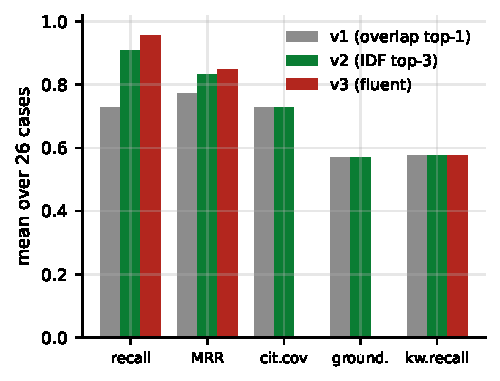
\includegraphics[width=\columnwidth]{aire_versions.pdf}
\caption{Deterministic three-version comparison over the 26-case suite.
The fluent-but-uncited version (v3) improves retrieval but destroys citation
coverage and groundedness, which the regression engine flags.}
\label{fig:versions}
\end{figure}

\subsection{Live LLM Results}
The same suite is then run with a real generator: an OpenAI-compatible
client calling Gemini 2.5 Flash (temperature 0) over the same local
retriever, under a prompt contract requiring per-sentence
\texttt{[doc:id]} citations and abstention when the context does not answer
the question. Calls are rate-limited by a pacing sleep that runs outside
the timed region, so latency metrics measure the system rather than the
limiter; token usage is recorded from API responses
(\texttt{token\_source} = \texttt{api}).

Against deterministic v2 (Table~\ref{tab:live},
Fig.~\ref{fig:live}), the LLM abstains correctly on all four unanswerable
cases (0.0 to 1.0) and its cited answers are fully supported by the lexical
judge (groundedness 1.0), while citation coverage slips slightly
(0.7273 to 0.6818) and operational cost grows by four orders of magnitude
in latency (0.30\,ms to 15{,}319.83\,ms per case) and seven-fold in tokens
(83 to 605 per case). Seventeen of 26 cases complete cleanly; six are
provider rate-limit failures (HTTP 429 surviving retries), recorded as
invocation errors. The comparison is a single run of a nondeterministic
system: it demonstrates the evaluator's behavior on a frontier model and
exposes the quality-versus-cost trade-off, but is not a statistical
benchmark.

\begin{table}[t]
\centering
\caption{Live Gemini 2.5 Flash versus deterministic v2 on the same 26-case
suite (regression-engine verdicts). One run; nondeterministic system.}
\label{tab:live}
\small
\begin{tabular}{@{}lrrl@{}}
\toprule
Metric & v2 (det.) & Gemini & Verdict \\
\midrule
abstention\_correct & 0.0000 & \textbf{1.0000} & improved \\
groundedness & 0.5682 & \textbf{1.0000} & improved \\
citation\_coverage & 0.7273 & 0.6818 & regressed \\
latency (ms/case) & 0.30 & 15{,}319.83 & regressed \\
tokens (per case) & 83 & 605 & regressed \\
\bottomrule
\end{tabular}
\end{table}

\begin{figure}[t]
\centering
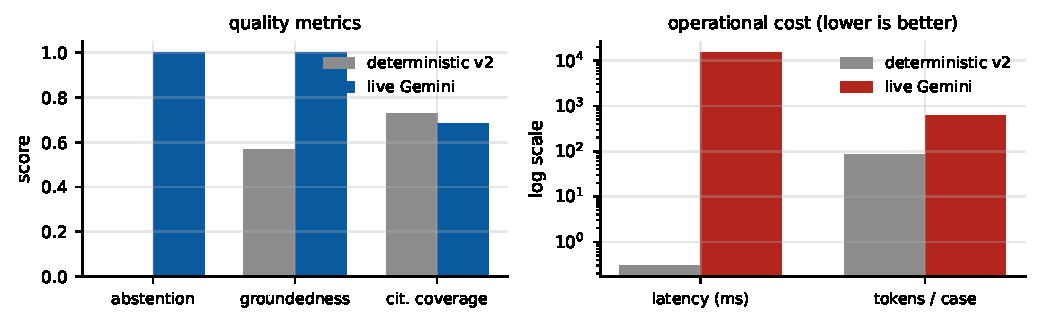
\includegraphics[width=\columnwidth]{aire_live.pdf}
\caption{Live LLM versus deterministic v2: quality gains (left) against
operational cost (right, log scale). The evaluator prices the trade-off
rather than issuing a single-number verdict.}
\label{fig:live}
\end{figure}

\section{Engineering Lessons}
Two reliability defects surfaced during development, both caught by the
deterministic harness and both fixed in the runner. First, provider errors
returned by the SUT as structured results were silently dropped: empty
answers from failed calls were classified as \emph{wrong abstentions}
instead of \emph{invocation errors}. The fix propagates the SUT's error
into the trace error field; the lesson is that error propagation must be
tested end to end. Second, the default 30-second invocation watchdog killed
14 of 26 live cases because thinking-mode generations run 30--90\,s; the
timeout became configuration, and the episode illustrates that reliability
parameters are part of the system under test. A third issue, a segmentation
bug that treated a trailing citation as its own unsupported sentence,
existed only in the evaluator and was invisible until the deterministic
harness made metric changes reproducible.

\section{Limitations}
(1) The groundedness metric is a lexical proxy and can be fooled in both
directions. (2) Keyword retrieval cannot decide answerability; the abstention
score distributions overlap measurably. (3) The deterministic responder is a
rule-based harness; it bounds what deterministic results can say about real
LLM behavior. (4) The live evaluation is a single run of 26 cases.
(5) Heuristic token counts are approximations by design. (6) The cost metric
uses a zero default price; real deployments must supply a price table.
(7) The corpus and case count are deliberately small; the machinery
(schema hashing, run isolation, attribution) is designed to scale but is
not demonstrated at scale here.

\section{Conclusion}
AIRE treats AI-system evaluation as a data problem: record validated traces
once, compute deterministic metrics, classify failures, and compare runs
with scale-free, direction-aware thresholds and per-case attribution. The
three-version demonstration shows the engine catching a regression
(groundedness 0.57 to 0.00) that reads as an improvement, and the live
evaluation shows it pricing a real trade-off: a frontier LLM fixes
abstention and grounding at four orders of magnitude higher latency. The
system's own boundaries (lexical grounding, lexical answerability, single-
run live results) are stated as part of the design. Code, committed result
files, and reports are available in the accompanying
repository.\footnote{\url{https://github.com/vaibhav3000/aire}}

\begin{thebibliography}{5}

\bibitem{vaswani2017attention}
A.~Vaswani, N.~Shazeer, N.~Parmar, J.~Uszkoreit, L.~Jones, A.~N. Gomez,
{\L}.~Kaiser, and I.~Polosukhin, ``Attention is all you need,'' in
\emph{Advances in Neural Information Processing Systems (NeurIPS)}, 2017,
arXiv:1706.03762.

\bibitem{lewis2020rag}
P.~Lewis, E.~Perez, A.~Piktus, F.~Petroni, V.~Karpukhin, N.~Goyal,
H.~K{\"u}ttler, M.~Lewis, W.~Yih, T.~Rockt{\"a}schel, S.~Riedel, and
D.~Kiela, ``Retrieval-augmented generation for knowledge-intensive NLP
tasks,'' in \emph{Advances in Neural Information Processing Systems
(NeurIPS)}, 2020, arXiv:2005.11401.

\bibitem{rajpurkar2016squad}
P.~Rajpurkar, J.~Zhang, K.~Lopyrev, and P.~Liang, ``SQuAD: 100{,}000+
questions for machine comprehension of text,'' in \emph{Proc. Conf. on
Empirical Methods in Natural Language Processing (EMNLP)}, 2016,
arXiv:1606.05250.

\bibitem{zheng2023judging}
L.~Zheng, W.-L. Chiang, Y.~Sheng, S.~Zhuang, Z.~Wu, Y.~Zhuang, Z.~Lin,
Z.~Li, D.~Li, E.~P. Xing, H.~Zhang, J.~E. Gonzalez, and I.~Stoica,
``Judging LLM-as-a-judge with MT-Bench and Chatbot Arena,'' in
\emph{Advances in Neural Information Processing Systems (NeurIPS)}, 2023,
arXiv:2306.05685.

\end{thebibliography}

\end{document}
